\chapter{2048}

\section{2048のルールと用語説明}
\label{sec:rule}
2048は, Gabrirle Cirulliによって公開された$1$人用のパズルゲームである~\cite{2048}.
ゲームは$16$マスからランダムに選ばれた$2$マスに$2$か$4$の数字タイルが置かれた盤面から始まる.
プレイヤが行うことは上下左右いずれかの方向を選択することである. 
プレイヤがある$1$つの方向を選ぶと, 盤面上のすべての数字タイルは選択した方向に向かってスライドして移動する.
スライドする数字タイルは空きマスを通過し, 異なる数字タイルの直前か盤面の端で停止する.
スライドして移動する際に$2$つの同じ数字のタイルが衝突すると, これらは合体してその合計の数字の$1$つのタイルへ変化し, プレイヤはその数値を得点として獲得する.
そのため, ゲームには$2$の累乗の数字タイルしか現れない.
図~\ref{fig:all_directions}にある盤面から上下左右を選択したときの, 数字タイルのスライドの仕方の具体例を示す.
\begin{figure}[t]
    \centering
    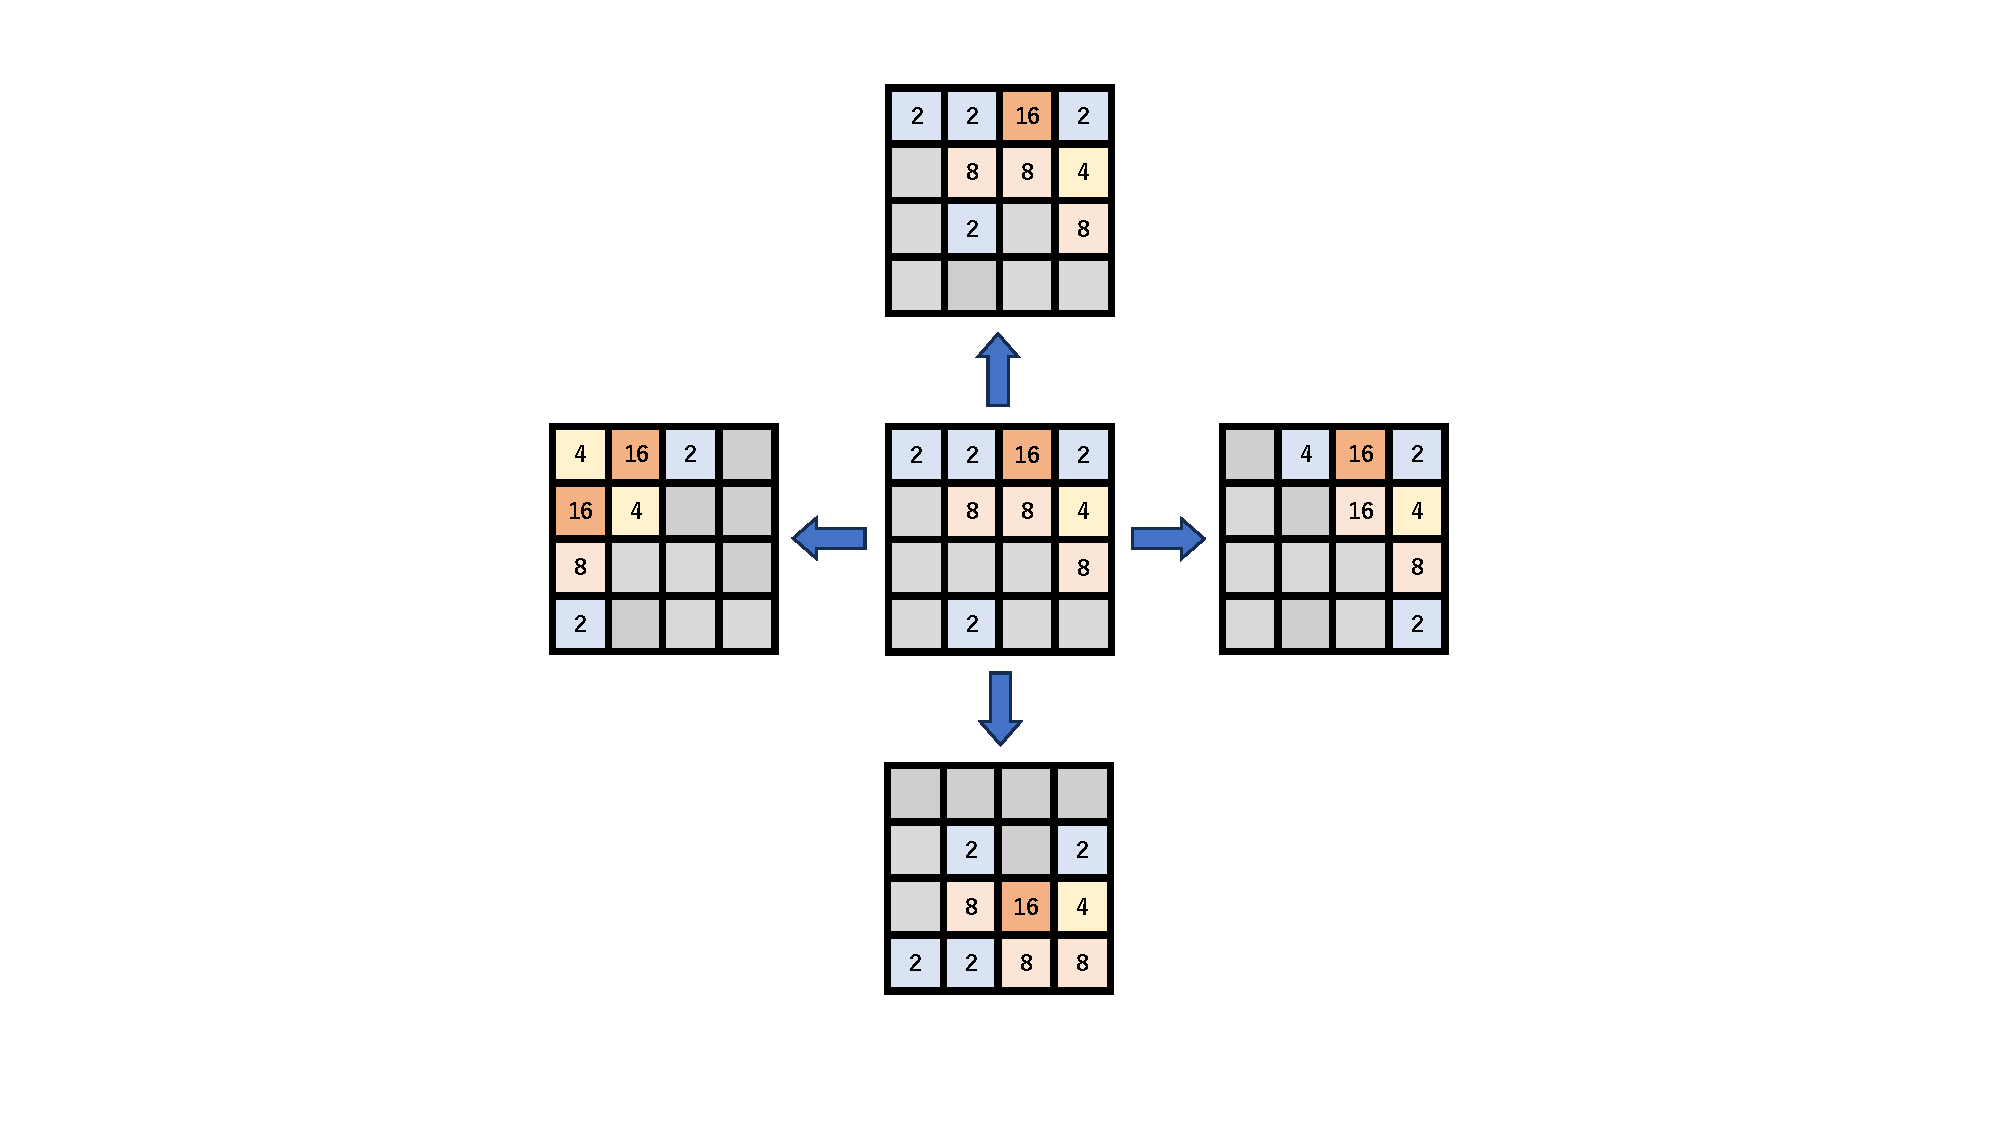
\includegraphics[width=0.8\linewidth{}]{figures/all_directions.pdf}
    \caption{上下左右それぞれへのスライドの例 \label{fig:all_directions}}
\end{figure}

数字タイルのスライド後, 空きマスから等確率に選択されたある1マスに$90\%$の確率で$2$のタイルが, $10\%$の確率で$4$のタイルが置かれる. 
ゲームはプレイヤの行動による数字タイルのスライドと新たな数字タイルの出現を交互に繰り返して進行する.
盤面上の数字タイルが市松模様のようになると, プレイヤが選択可能な行動がなくなったときにゲームは終了する~(図~\ref{fig:terminal}を参照).
\begin{figure}[t]
    \centering
    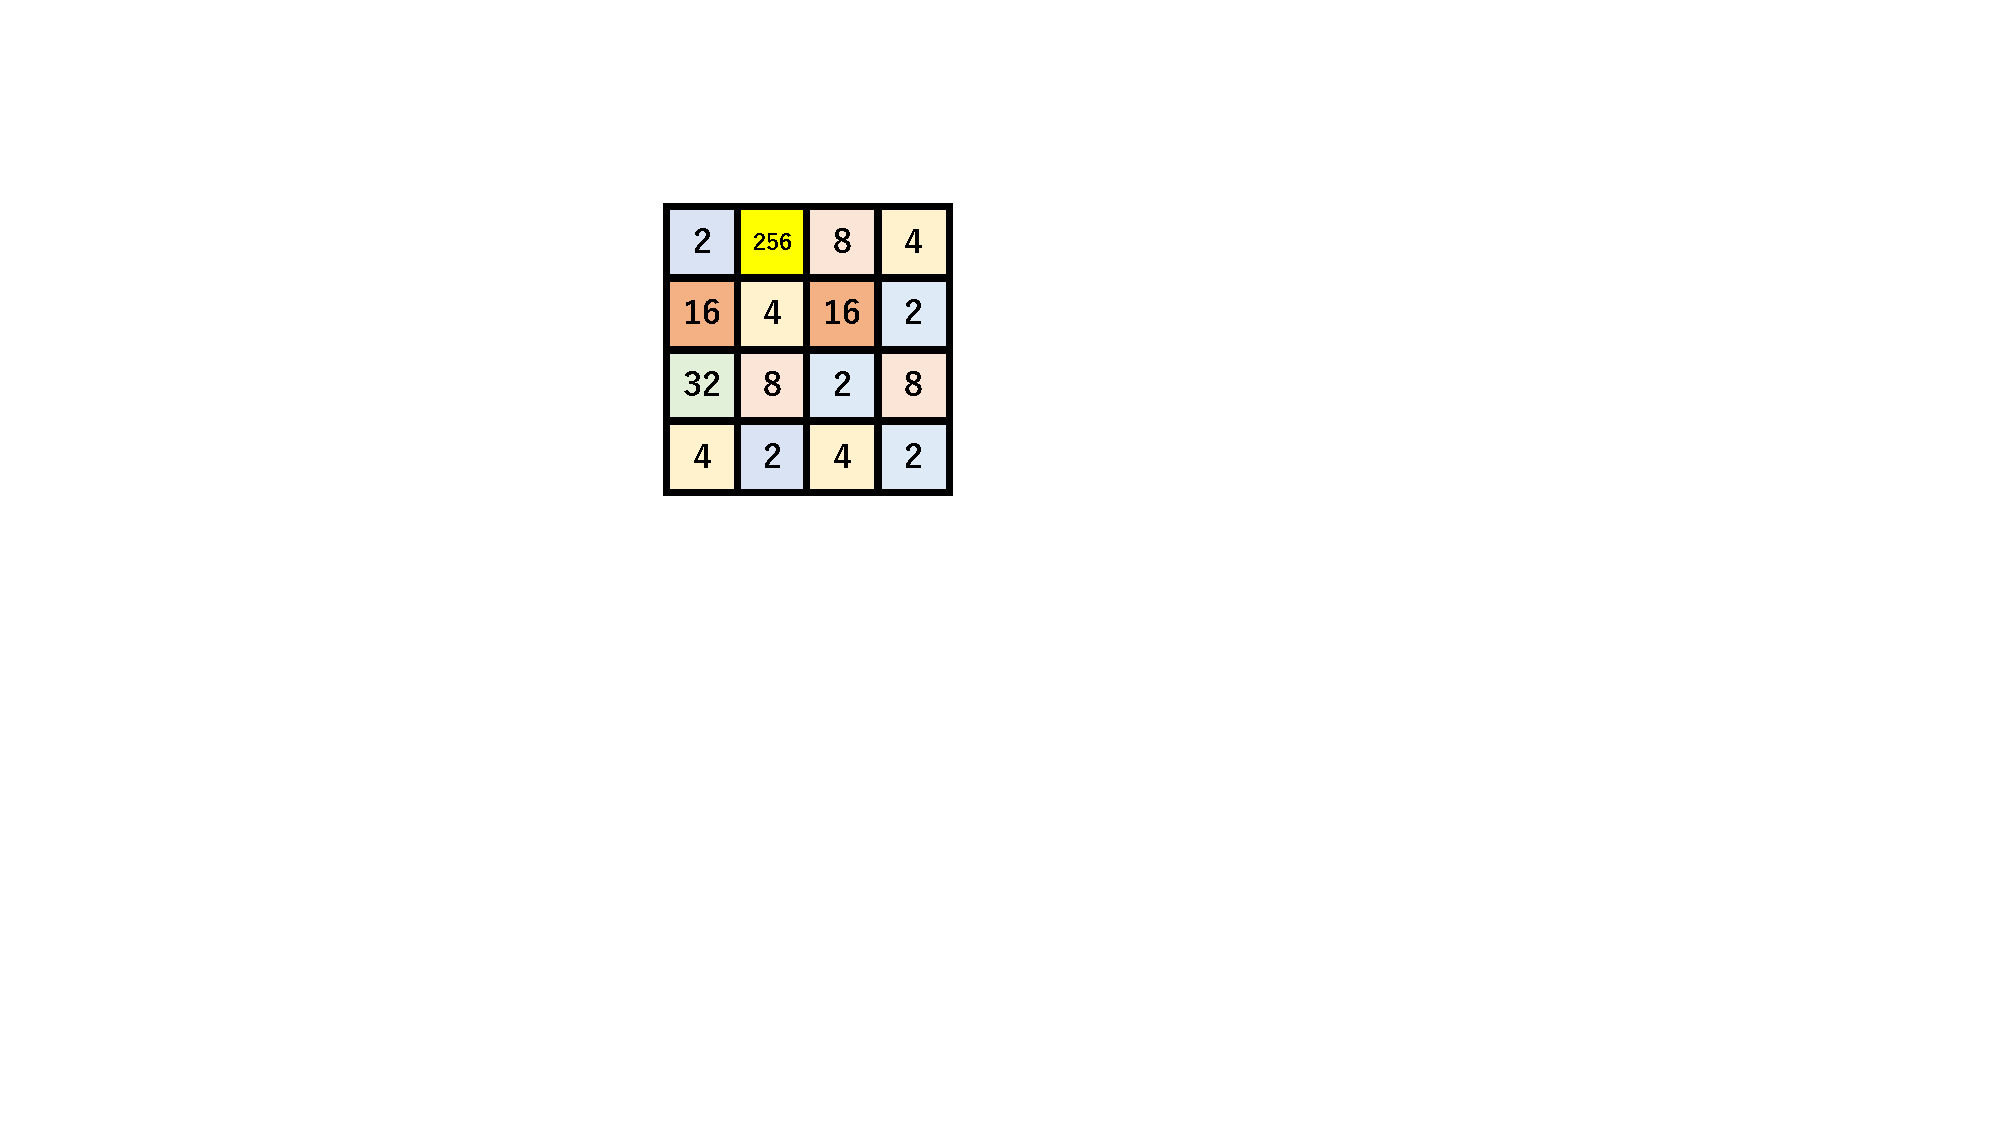
\includegraphics[width=0.2\linewidth{}]{figures/terminal_.pdf}
    \caption{終了状態の例 \label{fig:terminal}}
\end{figure}

ここでプレイヤが行動を選択する盤面を\textgt{状態}, 行動を選択して新たな数字タイルが出現する直前の盤面を\textit{afterstate}と呼ぶ.
図~\ref{fig:transition}に状態$s$からafterstate $s'$を経由して, 次の状態$s_{\text{next}}$に遷移する例を示す.

\begin{figure}[t]
    \centering
    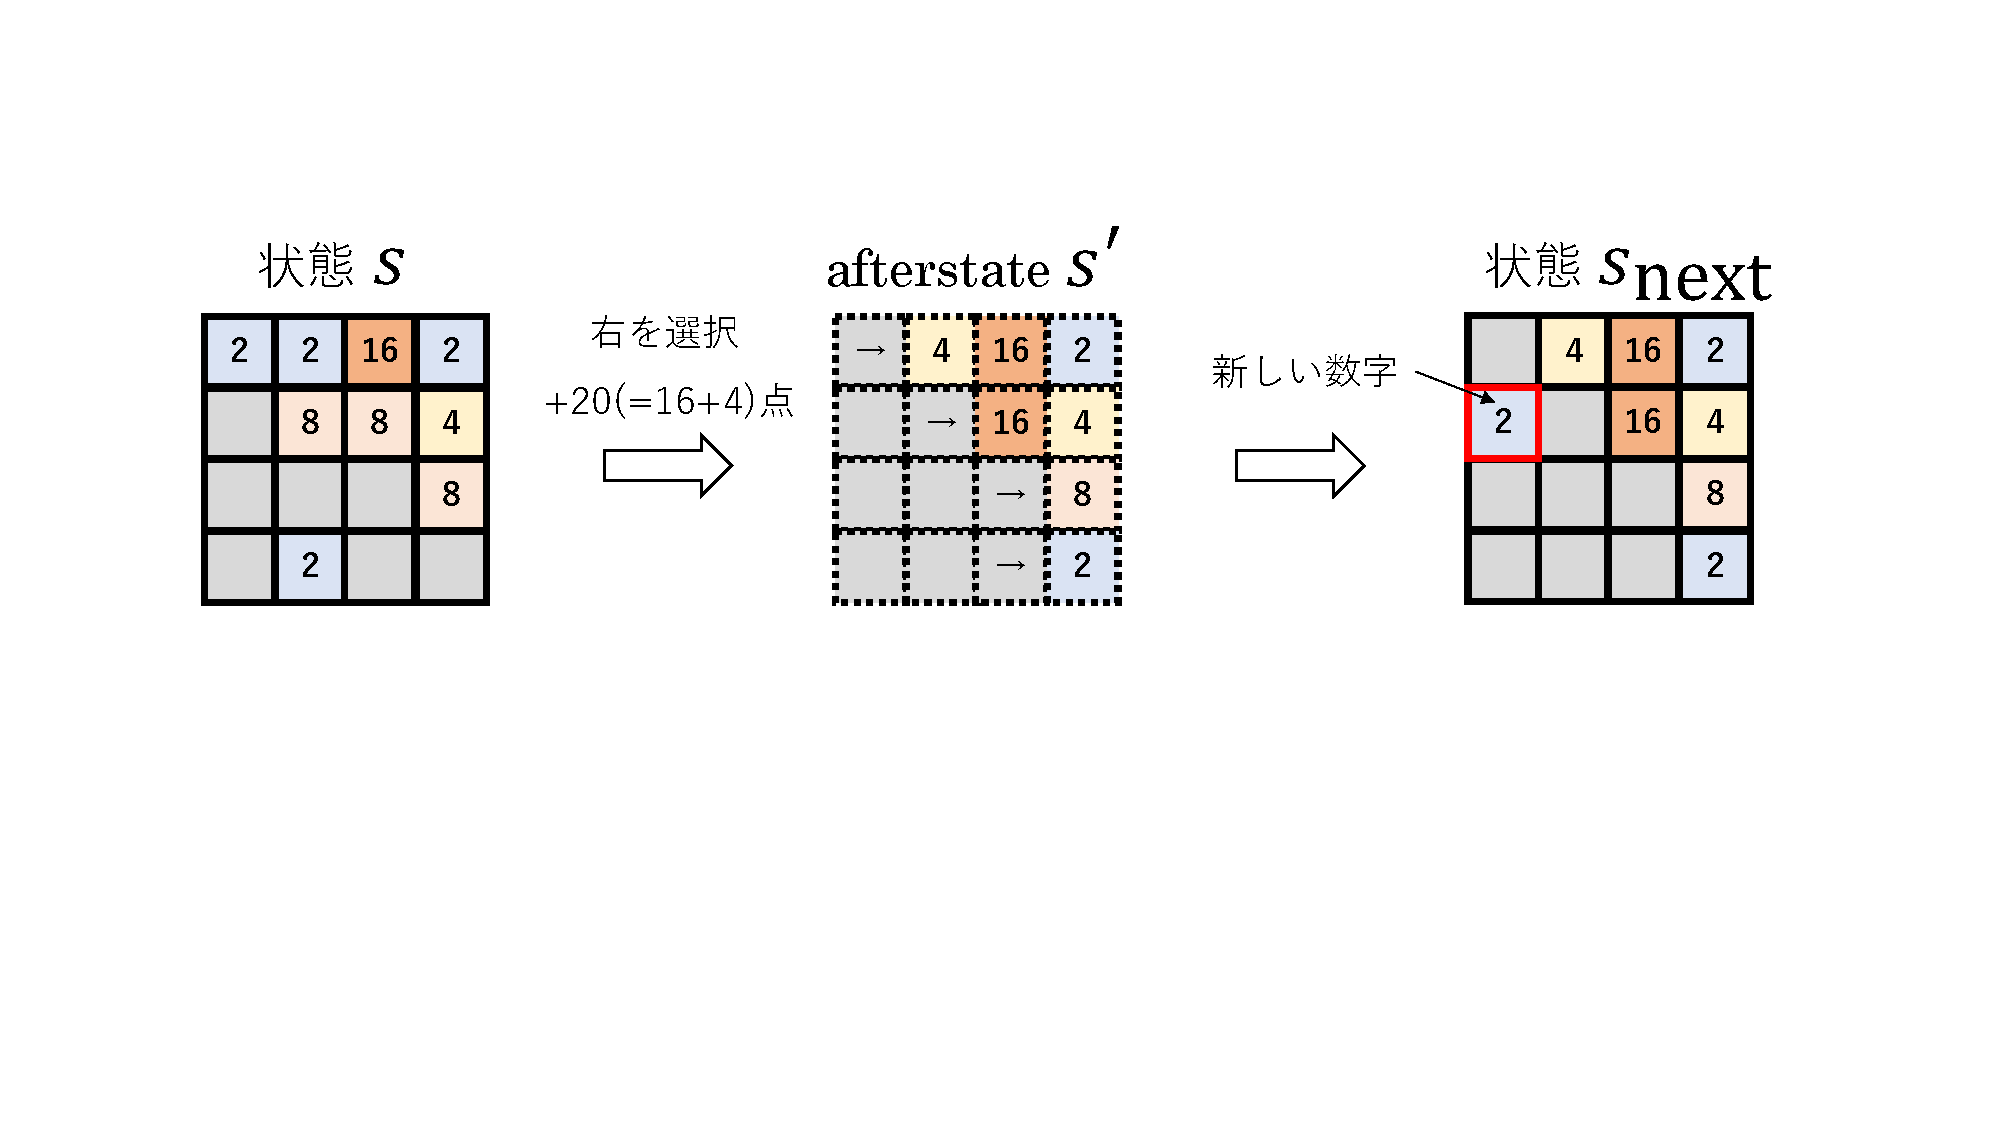
\includegraphics[width=\linewidth{}]{figures/transition_.pdf}
    \caption{状態遷移の例 \label{fig:transition}}
\end{figure}

プレイヤの一般的な目標はゲームのタイトルが示す$2^{11}=2048$のタイルを完成させることだが, それ以降もゲームを続けることができる.

\section{ゲームの進行と時刻}
\label{sec:property}
2048はゲームの性質上, 状態からafterstateへの遷移において盤面上の数字タイルの合計値は不変である~(図~\ref{fig:all_directions}を参照).
盤面上の数字タイルの合計値はafterstateから次の状態への遷移においてのみ変化する.
新しい数字タイルとして$2$か$4$のタイルが出現することで, 数字タイルの合計値はその値の分だけ必ず増加する.
すなわちプレイヤが$1$回行動するたびに, 盤面上の数字タイルの合計値は$2$か$4$ずつ単調に増加する.

よって盤面上の数字タイルの合計値をゲームの進行度合いとして用いることができる.
以降これを\textgt{時刻}と呼ぶ.
例えば図~\ref{fig:transition}では時刻$2\times4+4+8\times3+16=52$の状態$s$が時刻$52+2=54$の状態$s_{\text{next}}$に遷移している.
ゲームの時刻はプレイヤが行動するたびに必ず増加するため, 2048はサイクルの出現しないゲームであることがわかる.



\subsection{ゲームの終了状態}

またゲームの開始盤面をまとめて初期状態と呼ぶことにする.